%!TEX program = xelatex
%!TEX TS-program = xelatex
%!TEX encoding = UTF-8 Unicode

\documentclass[12pt]{article} %这个我就不多说了,头文件
\usepackage{url} %这个我也不多说了
\usepackage{fontspec,xltxtra,xunicode} %最新的mactex都有
\defaultfontfeatures{Mapping=tex-text}
\setromanfont{Heiti SC} %设置中文字体
\XeTeXlinebreaklocale “zh”
\XeTeXlinebreakskip = 0pt plus 1pt minus 0.1pt %文章内中文自动换行,可以自行调节

\newfontfamily{\H}{Songti SC} %设定新的字体快捷命令
\newfontfamily{\E}{Weibei SC} %设定新的字体快捷命令


\addtolength{\textwidth}{2cm}
\addtolength{\hoffset}{-1cm}
\addtolength{\marginparwidth}{-1cm}
\addtolength{\textheight}{2cm}
\addtolength{\voffset}{-1cm}

\usepackage{amsmath}
\usepackage{cases}
\usepackage{listings}
\usepackage{xcolor}
\usepackage{float}
\usepackage{graphicx}
\usepackage{subfigure}
\usepackage{cite}

\title{Ising模型}
\author{丁历杰}
\date{}
\begin{document}
\lstset{
numbers=left,
numberstyle= \tiny,
keywordstyle= \color{ blue!70},commentstyle=\color{red!50!green!50!blue!50},
%frame=shadowbox,
rulesepcolor= \color{ red!20!green!20!blue!20}
}
\numberwithin{equation}{subsection}

\maketitle
\section{模型简介}
对于一系列晶格点的集合S,其中每一个晶格点都有一个所有与之相邻的晶格点的集合T,并另这些晶格点形成一个d维的晶格.对于每一个晶格点$k\in S$都有一个离散参数$\sigma_k \ in (+1,-1)$,代表每一个晶格点的自旋.而所有的离散参数集合$\Sigma \equiv {\sigma_k}_{k\in S}$为体系的自旋组态.
对于每两个相邻的晶格点$i,j \in S$,引入相互作用参数$J_{ij}$,并假设每个晶格点都和外加磁场$h_j$作用,则体系的Hamilton量可以写作:
\begin{equation}
\label{equ: Hamilton}
H(\sigma) = -\sum_{\langle i,j \rangle}J_{ij}\sigma_{i}\sigma_{j}-\mu \sum_{j}h_{j}\sigma_{j}
\end{equation}
其中$\langle i,j \rangle$代表i和j晶格点是相邻的,在Hamilton量的计算中只对每一堆晶格点计算一次.第二项是磁场与自旋的相互作用能,$\mu$是晶格点的磁矩.

Ising模型\cite{Ising_wiki}是统计力学中关于相变的较为基础的模型.它的最早的提出者是Wilhelm Lenz(1920).后来他让他的学生Ernst Ising对一维的Ising模型进行求解,但是并没有发现相变现象,因此也没有得到更多物理学家的关注.随后,Lars Onsager于1944年对二维的Ising模型进行了解析求解($H=0$的情况,$H\neq0尚无解析接$),并同时发现了二维Ising模型中的相变现象,从而引起了更多学者的关注.之后,随着Landau、Ginzburg等人的努力.人们发现了Ising模型与量子场论之间的联系,并创立了平行的统计场论.
\section{统计分析}
在Ising模型中,粒子数固定,粒子自旋(广义坐标)的取值范围固定,所以如果定义了温度T固定(达到热平衡)的话,那么有其组成的系综就是一个正则系综.其相空间中的概率分布为Boltzman分布:
\begin{equation}
\label{equ: Distribution}
\begin{aligned}
P_{T}(\Sigma) = \frac{e^{-H(\Sigma)/(k_{B}T)}}{Z} \\
Z = \sum_{\Sigma}e^{-H(\Sigma)/(k_{B}T)}
\end{aligned}
\end{equation}

因而对于任何一个可观测量$\Omega$,都可以写作:
\begin{equation}
\label{equ: Obseration}
\langle \Omega \rangle = \sum_{\Sigma}\Omega(\Sigma)P_{T}(\Sigma)
\end{equation}

\subsection{关于参数的讨论}
在Hamilton量中参数$J_{ij}$和$h_{i}$值得进一步探讨.
$$
\begin{cases}
    J_{ij}>0, 称该体系为铁磁性 \\
    J_{ij}<0, 称该体系为反铁磁性 \\
    J_{ij}=0, 说明晶格点间无相互作用
\end{cases}
$$
$$
\begin{cases}
    h_i>0, 则晶格点i趋于正向 \\
    h_i<0, 则晶格点i趋于反向 \\
    h_i=0, 则说明没有外加力长作用
\end{cases}
$$

\subsection{模型的简化}
常见的简化模型为:
\begin{enumerate}
    \item 没有外加力场作用: $H(\sigma) = -\sum_{\langle i,j \rangle}J_{ij}\sigma_{i}\sigma_{j}$
    \item 进一步的,所有晶格相互作用是相同的: $H(\sigma) = -J\sum_{\langle i,j \rangle}\sigma_{i}\sigma_{j}$
\end{enumerate}

\subsection{一维Ising模型解析解}
对于正则系综,体系的特征函数是Helmoholtz自由能F,达到平衡态时F取极小值.\cite{热统汪志诚}
\begin{equation}
\label{equ: Free_energy}
F = -k_{B}T\ln Z
\end{equation}

\subsubsection{h=0}
对于h=0的情况,可以在一维自由边界条件下进行求解,N个自旋排成一列,端点之间没有相互作用,此时系统的Hamilton量为:
\begin{equation}
\label{equ: Hamilton_1D_H0}
E(\Sigma) = -J\sum_{i=1}^{N-1}\sigma_{i}\sigma_{i+1} = -J(\sigma_1\sigma_2+\dots+\sigma_{N-1}\sigma_N)
\end{equation}
令$K\equiv J/K_{B}T, \sigma_{i}'=\sigma_{i}\sigma_{i-1} (i\leq 2)$,则系统的配分函数:
\begin{equation}
\label{equ: Z_1D_H0}
Z = \sum_{\sigma_1,\dots,\sigma_N}e^{K(\sigma_1\sigma_2+\dots+\sigma_{N-1}\sigma_N)} = 2\prod_{i=2}^{N}\sum_{\sigma_{i}'}e^{K\sigma_{i}'} = 2[e^{K}+e^{-K}]^{N-1}
\end{equation}
进而由\eqref{equ: Free_energy}式,对于$N\rightarrow \infty$每个粒子的平均自由能$f = \frac{F}{N} = -k_{B}T\ln [e^{K}+e^{-K}]$,除了$T=0,\infty$外f及其温度的高阶导数没有奇点,所以不存在相变.

\subsubsection{$h\neq0$}
对于$h\neq0$的情况,可以周期边界条件进行求解,,此时系统的Hamilton量为:
\begin{equation}
\label{equ: Hamilton_1D_H}
E(\Sigma) = -J\sum_{i=1}^{N}\sigma_{i}\sigma_{i+1} - H\sum_{i=1}^{N}\sigma_i
\end{equation}
令$K\equiv J/K_{B}T, I = H/K_{B}T$,则系统的配分函数:
\begin{equation}
\label{equ: Z_1D_H}
Z = \sum_{\sigma_1,\dots,\sigma_N}e^{I\sigma_1}e^{K\sigma_1\sigma_2}e^{I\sigma_2}e^{K\sigma_2\sigma_3}\dots^{I\sigma_N}e^{K\sigma_N\sigma_1}
= \sum_{\sigma_1,\dots,\sigma_N}V_{\sigma_1,\sigma_2}V_{\sigma_2,\sigma_3}\dot sV_{\sigma_N,\sigma_1}
\end{equation}
其中的$V_{\sigma_i,\sigma_j} = e^{\frac{I\sigma_i}{2}}e^{K\sigma_i\sigma_j}e^{\frac{I\sigma_j}{2}}$ 可以视$\sigma_i,\sigma_j$的取值视为矩阵:
$$
V=
\left[
\begin{matrix}
    e^{K+I}&e^{-K+I} \\
    e^{-K+I}&e^{K-I}
\end{matrix}
\right]
 $$
进而:
$$Z = \sum_{\sigma_1,\dots,\sigma_N}\langle\sigma_1|V|\sigma_2\rangle\langle\sigma_2|V|\sigma_3\rangle\dots\langle\sigma_N|V|\sigma_1\rangle = \sum_{\sigma_1}\langle\sigma_1|V^{N}|\sigma_1\rangle = Tr V^N = \lambda_{+}^N+\lambda_{-}^N $$
$$\lambda_{\pm} = e^K\cosh I \pm \sqrt{e^{2K}\sinh{I}^2+e^{-2K}}$$
进而由\eqref{equ: Free_energy}式,对于$N\rightarrow \infty$每个粒子的平均自由能
$$f = \frac{F}{N} \approx -k_{B}T\ln e^K\cosh I + \sqrt{e^{2K}\sinh{I}^2+e^{-2K}} (\lambda_{+}>\lambda_{-})$$
同样地除了$T=0,\infty$外f及其温度的高阶导数没有奇点,所以不存在相变.

\section{模拟分析}
下面对二维的Ising模型进行模拟计算:
所采用的Hamilton量
\begin{equation}
\label{equ: Hamilton_2D}
E(\Sigma) = -J\sum_{i,j}\sigma_{i,j}(\sigma_{i-1,j}+\sigma_{i+1,j}+\sigma_{i,j-1}+\sigma_{i,j+1}) - H\sum_{i,j}\sigma_{i,j}
\end{equation}

\subsection{程序结构} % (fold)
\label{sec:程序结构_}
为了加强程序的模块化,编写了如下的类来进行算法实现。
\begin{lstlisting}[language=C++]
class ising
{
private:
    struct neighbor
    {
        int spin;
        int ux, uy;
        int dx, dy;
        int lx, ly;
        int rx, ry;
    } **mark;
    int size;
    int up_count;
    double up_rate;
    double T;
    double J;
    double H;
    /*
    neighbor is a struct for every lattice info storage
    and mark is a 2 dimensional neighbor pointer
     which contain all the map
    size is the size of the table
    m is the average spin
    T is the temperature
    h is the megnetic field
     */
public:
    ising(  int size_,
            double up_rate_,
            double T_,
            double J_,
            double H_);
    void refresh(   double T_,
                    double J_,
                    double H_);
    //refresh the object's parameters  as you wish!
    //will set all spins up
    void reset( double T_,
                double J_,
                double H_);
    //reset the object's parameters as you wish
    //will not reset spins' direction


    int get_size(); //size getting
    int get_up_count(); //up_count getting
    double get_up_rate(); //up_rate getting
    double get_T();
    double get_J();
    double get_H();
    double get_z(); //z = (exp(2J/T)−1)
    double get_energy(); //get the energy
    double get_m(); //get m = average(s)

    //Algorithms
    void metropolis(int steps);
    void swendsen_wang(int steps);
    void wolff(int steps);
    void worm(int steps);



    //output data methods
    void output_mark_pos(std::string filename);
    void output_n_E_m(  int init_step,
                        int steps,
                        int per_step,
                        std::string filename);
    void output_T_E_C_m(int equi_step,
                        int ave_step,
                        int step_per_ave,
                        double T_start,
                        double T_end,
                        double delta_T,
                        std::string filename);
    void output_H_E_C_m(int equi_step,
                        int ave_step,
                        int step_per_ave,
                        double H_start,
                        double H_end,
                        double delta_H,
                        std::string filename);

    void output_T_H_E_C_m(int equi_step,
                          int ave_step,
                          int step_per_ave,
                          double T_start,
                          double T_end,
                          double delta_T,
                          double H_start,
                          double H_end,
                          double delta_H,
                          std::string filename);
    void output_H_loop_E_C_m(int equi_step,
                             int ave_step,
                             int step_per_ave,
                             double H_start,
                             double H_end,
                             double delta_H,
                             std::string filename);
};
\end{lstlisting}

\subsection{模拟算法}
\paragraph{细致平衡}
由主方程\cite{Master_equ}可以的到细致平衡解:
\begin{equation}
\label{equ: Detaled_balance}
\frac{P(x\rightarrow x')}{P(x'\rightarrow x)} = \frac{P(x')}{P(x)}
\end{equation}

\subsubsection{Metropolis}
Metropolis算法\cite{Metropolis_wiki}是一种Markov Chain Monte Carlo(MCMC)算法,由Metropolis等人在1953年提出\cite{Metropolis:1953vj}.

\paragraph{算法导出}
为了得到Metropolis算法,将细致平衡中的转移概率分为两个部分:提议概率$g(x\rightarrow x')$和接受概率$A(x\rightarrow x')$.
$$P(x\rightarrow x') = g(x\rightarrow x')A(x\rightarrow x')$$
进而:
$$
\frac{A(x\rightarrow x')}{A(x'\rightarrow x)} = \frac{P(x')}{P(x)}\frac{g(x'\rightarrow x)}{g(x\rightarrow x')}
$$
选择满足上述条件的接受概率,便可满足细致平衡条件,而Metropolis算法为:
\begin{equation}
\label{equ: Metropolis}
A(x\rightarrow x') = \min\left(1,\frac{P(x')}{P(x)}\frac{g(x'\rightarrow x)}{g(x\rightarrow x')}\right)
\end{equation}

\paragraph{具体算法}
在本次的模拟中,具体采用的算法是.
\begin{enumerate}
    \item 以均匀分布随机选取一个晶格点,计算它的局域能量$E_{old}$
    \item 反转它,计算新的局域能量$E_{new}$
    \item 以概率$\min(1,e^{-(E_{new}-E_{old})/k_{B}T})$接受新的状态
    \item 重复上述步骤
\end{enumerate}

\subsubsection{Swendsen-Wang}
Swendsen-Wang方法是处理临界慢化问题的一种加速方法,整个系统被分为一系列的团簇集团,每个团簇集团再被随机的赋予新的自旋值.由Swendsen和Wang于1987年提出\cite{Swendsen:1987eq},具体的团簇产生由逾渗模型中的Hoshen-Kopelman的逾渗集团标记法\cite{Hoshen:1976vg}产生.

\paragraph{具体算法}
\begin{enumerate}
    \item 产生初始自旋构型(比如可以先由Metropolis法热化)
    \item 进行自旋键逾渗变换
    \item 由Hoshen-Kopelman的逾渗集团标记法将所有联键的集团逐一标识
    \item 对每个集团分别产生(+1,-1)的随机整数,赋予该集团中所有的晶格点该自旋值.
    \item 重复2至4步
\end{enumerate}

\subsubsection{Worff}
Worff算法也是一种集团算法,由Worff于1989年提出\cite{Wolff:1988uh}.与Swendsen-wang
算法所不同的是,Worff算法一次只反转一个集团,并且集团的产生并不是连接所有的键逾渗中的联键集团.\cite{Krauth:2003ts}

\paragraph{具体算法}
\begin{enumerate}
    \item 选取一个随机晶格点i,将其放入集团标记数组C
    \item 遍历所有未遍历过的C中晶格点的邻居晶格点j,
    \item 如果$\sigma_{j} = \sigma_{i}$, 则以$p=1-\exp(-2J/k_{B}T)$的概率接受它加入C(若拒绝了之后便不会再遍历到)
    \item 当C中晶格点的邻居中没有未遍历过的了,C中所有的自旋反向.
    \item 重复上述步骤
\end{enumerate}

\subsection{模拟分析}
不同温度下,由于涨落的不同,从而构成平衡态的状态大不相同.

\paragraph{可以看到不同温度下平均磁矩m随演化步数的变化}
\begin{figure}[hbt]
    \caption{m随演化步数的变化}
    \setcounter{subfigure}{0}
    \begin{center}
        \subfigure[T=1.50,J=1,H=0]{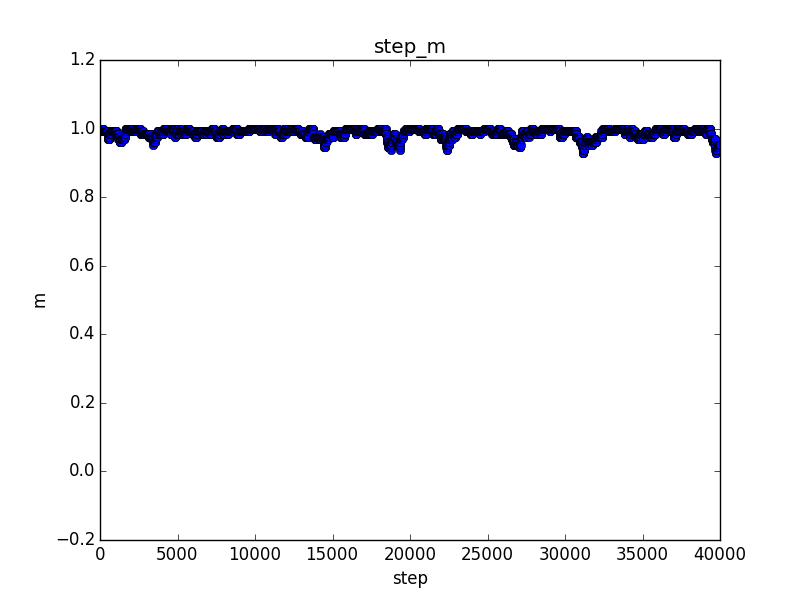
\includegraphics[width = 5cm]{n_m_16_T1.5_J1_H0.png}}
        \subfigure[T=2.25,J=1,H=0]{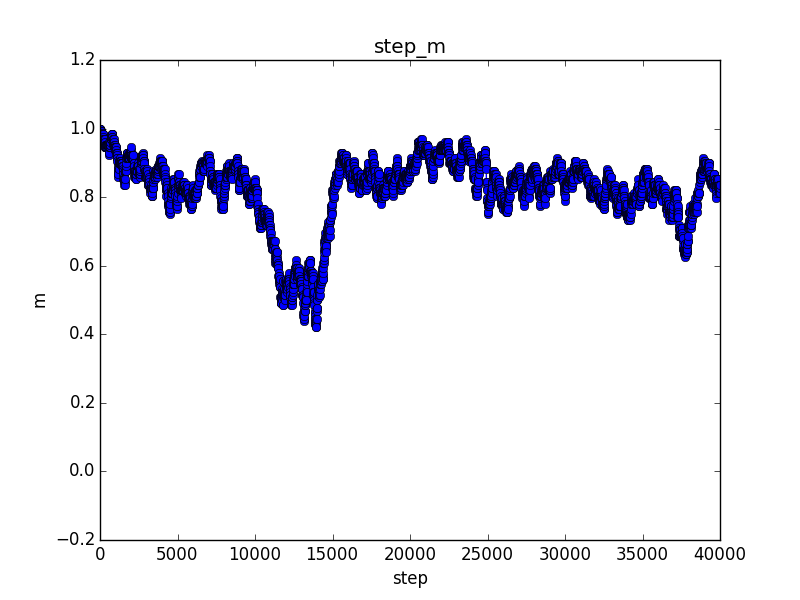
\includegraphics[width = 5cm]{n_m_16_T2.25_J1_H0.png}}
        \subfigure[T=4,J=1,H=0]{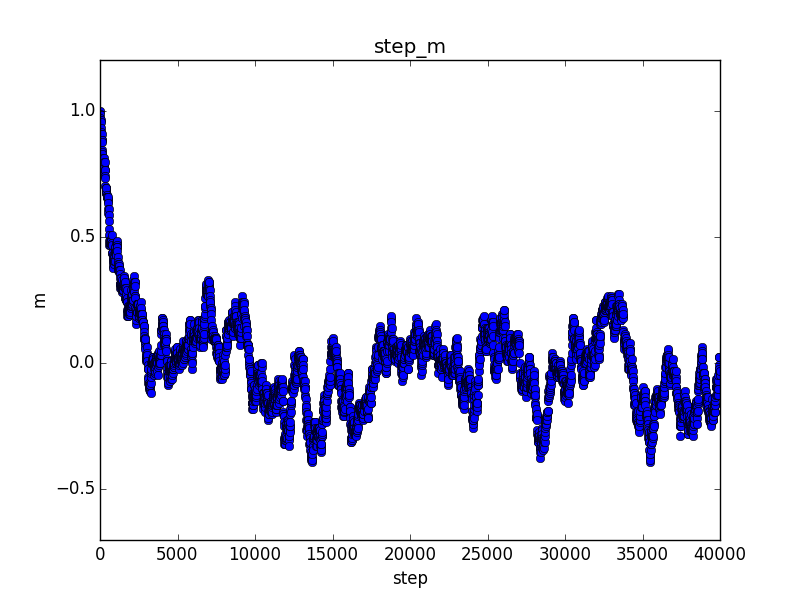
\includegraphics[width = 5cm]{n_m_16_T4_J1_H0.png}}

    \end{center}
\end{figure}

\clearpage
\paragraph{演化了1e8步后体系稳态状态}
\begin{figure}[hbt]
    \caption{体系稳态状态}
    \setcounter{subfigure}{0}
    \begin{center}
        \subfigure[T=1.50,J=1,H=0]{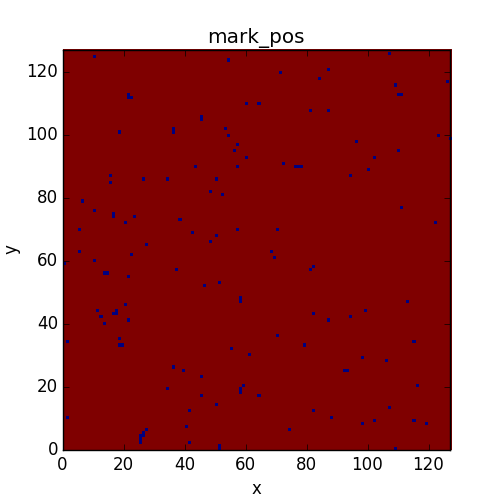
\includegraphics[width = 5cm]{mark_pos_128_T1.5_J1_H0.png}}
        \subfigure[T=2.25,J=1,H=0]{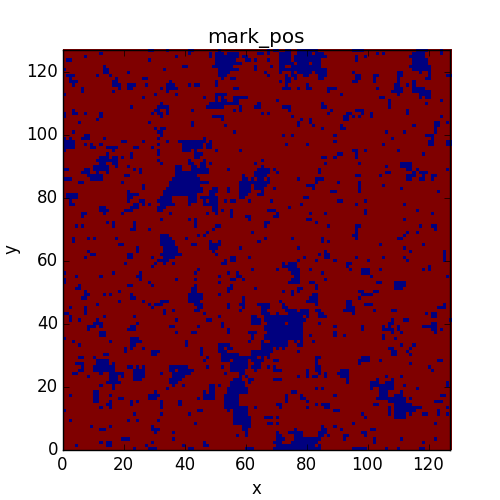
\includegraphics[width = 5cm]{mark_pos_128_T2.25_J1_H0.png}}
        \subfigure[T=4,J=1,H=0]{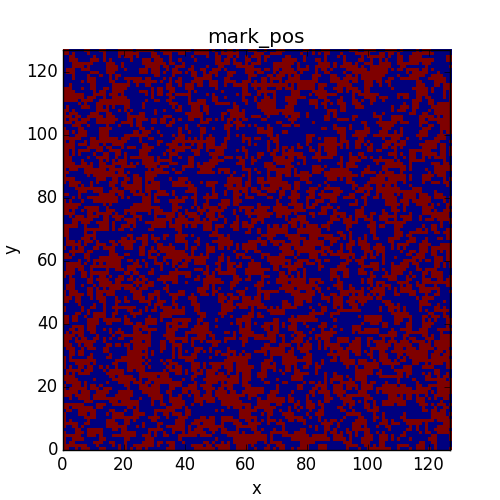
\includegraphics[width = 5cm]{mark_pos_128_T4_J1_H0.png}}
    \end{center}
\end{figure}


\paragraph{而平均自旋m关于参数(H,T)的变化($Size = 64\time64$)}

\begin{figure}[hbt]
    \caption{m关于(H,T)变化}
    \setcounter{subfigure}{0}
    \begin{center}
        \subfigure[H\_T\_m]{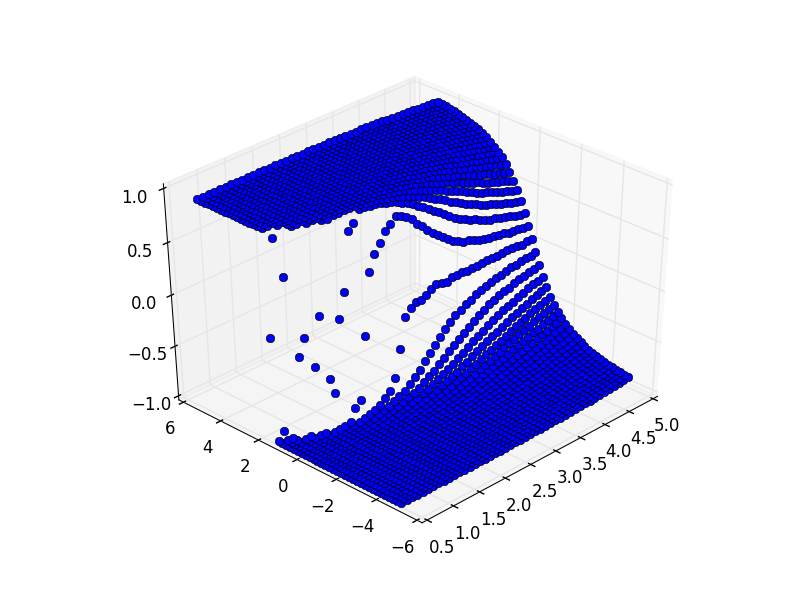
\includegraphics[width = 7cm]{H_T_m_fig.png}}
        \subfigure[H\_T\_E]{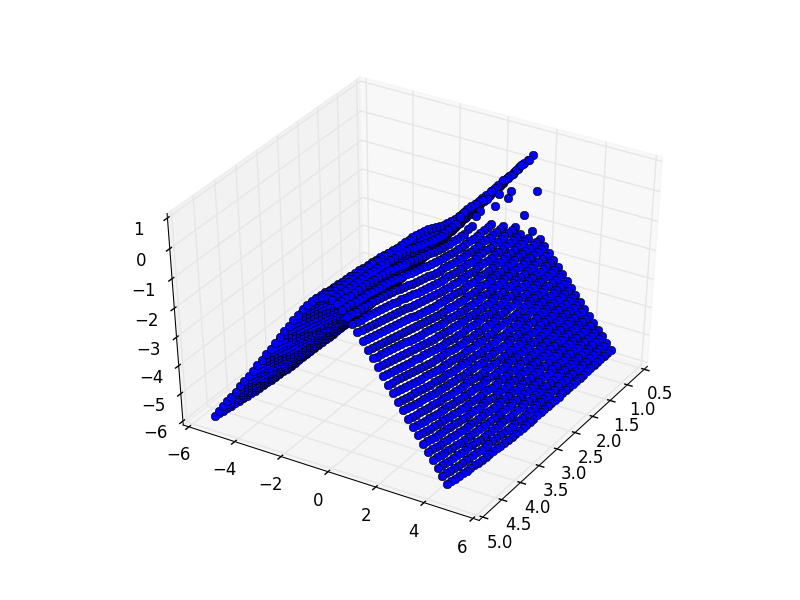
\includegraphics[width = 7cm]{H_T_E_fig.png}}
    \end{center}
\end{figure}
可以看到,在T较小(<$T_c$)的部分,m随H的变化出现了断裂,也就是说存在一级相变,而在较大的T出,都是连续的,所以是存在二级相变.E页同样出项了断裂.


\subsubsection{二级相变}
随着温度的改变,观察平衡态统计量的变化(E:平均能量,C:比热,平均自旋),模拟的大小为$128\times128$.

\paragraph{H=0时,随温度的变化}
\begin{figure}[hbt]
    \caption{H=0,随温度变化}
    \setcounter{subfigure}{0}
    \begin{center}
        \subfigure[T\_E,J=1,H=0]{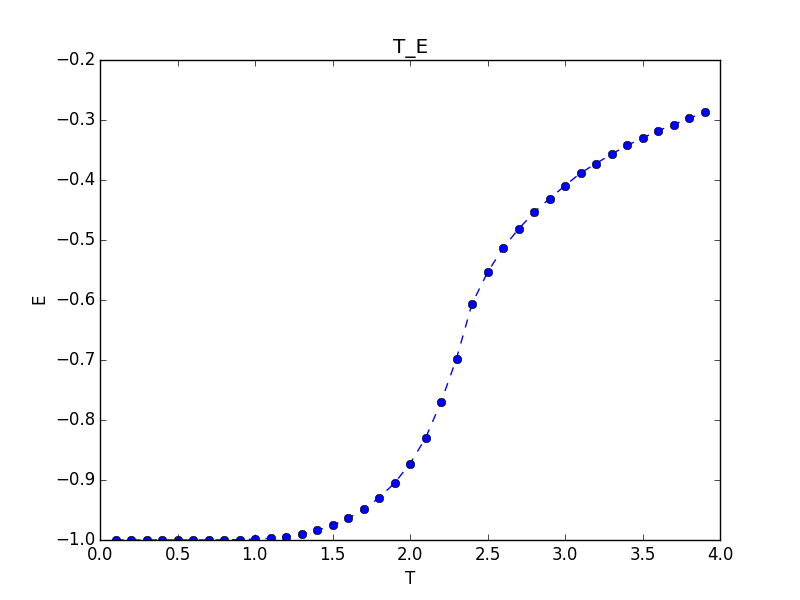
\includegraphics[width = 5cm]{T_E_128_J1_H0.png}}
        \subfigure[T\_C,J=1,H=0]{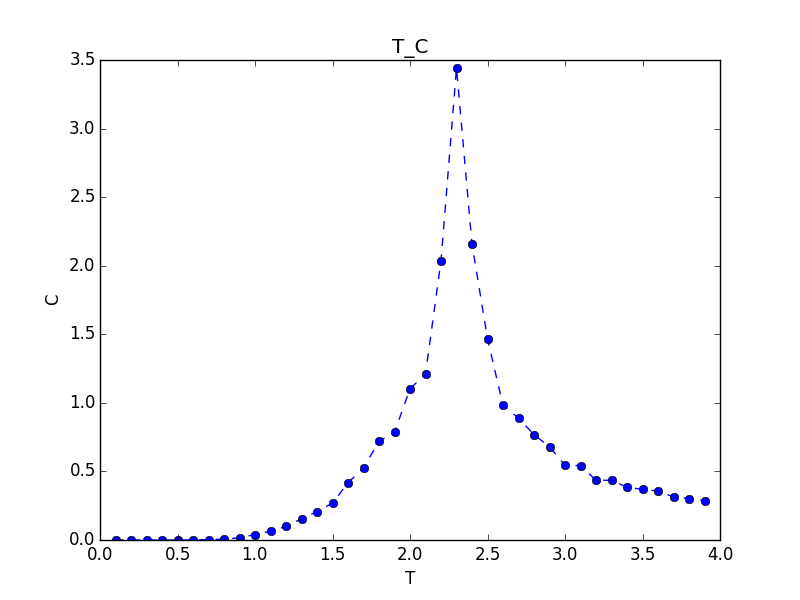
\includegraphics[width = 5cm]{T_C_128_J1_H0.png}}
        \subfigure[T\_m,J=1,H=0]{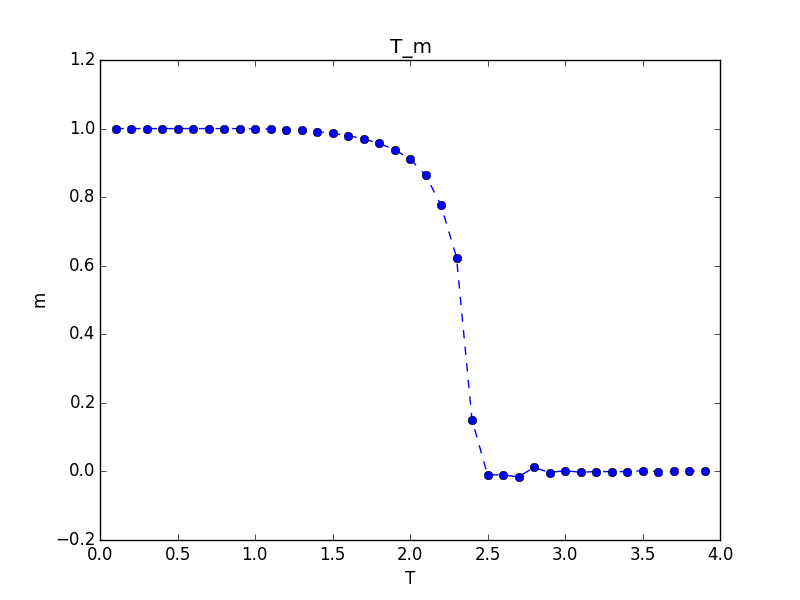
\includegraphics[width = 5cm]{T_m_128_J1_H0.png}}
    \end{center}
\end{figure}

\paragraph{$T>T_c$时,随磁场的变化}
\begin{figure}[hbt]
    \caption{$T>T_c$,随磁场变化}
    \setcounter{subfigure}{0}
    \begin{center}
        \subfigure[H\_E,T=4,J=1]{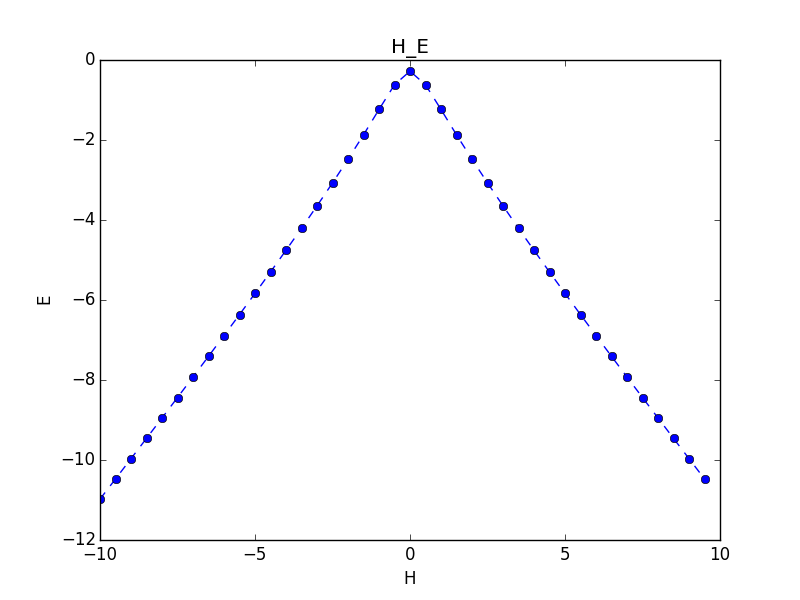
\includegraphics[width = 5cm]{H_E_128_T4_J1.png}}
        \subfigure[H\_C,T=4,J=1]{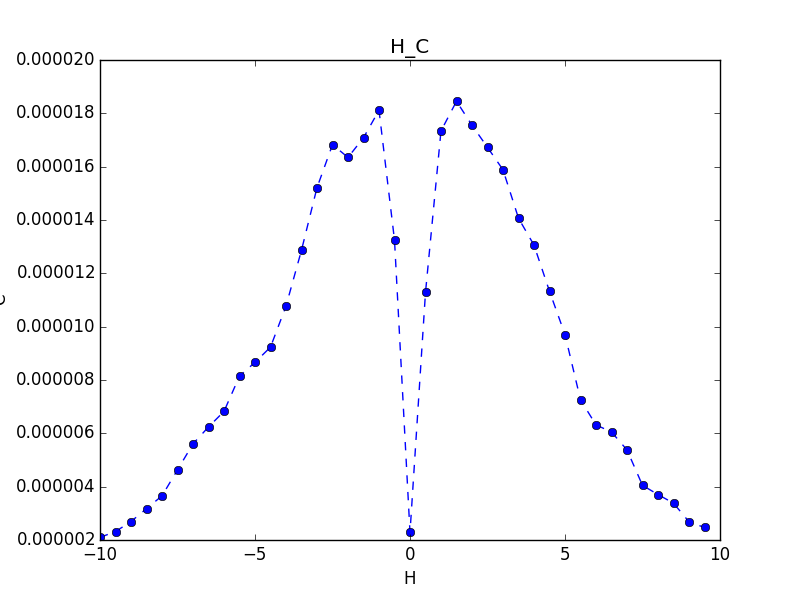
\includegraphics[width = 5cm]{H_C_128_T4_J1.png}}
        \subfigure[H\_m,T=4,J=1]{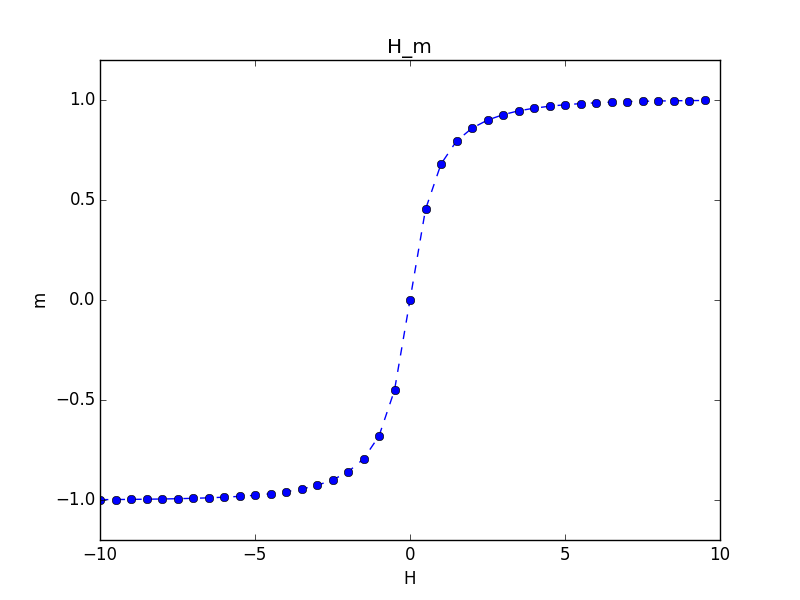
\includegraphics[width = 5cm]{H_m_128_T4_J1.png}}
    \end{center}
\end{figure}

\clearpage
\subsubsection{一级相变}
随着温度的降低,以及磁场的改变,体系将出项一级相变:
\paragraph{改变磁场,m随T的变化趋势改变}

\begin{figure}[hbt]
    \caption{m\_T趋势随磁场变化}
    \setcounter{subfigure}{0}
    \begin{center}
        \subfigure[J=1,H=-0.5]{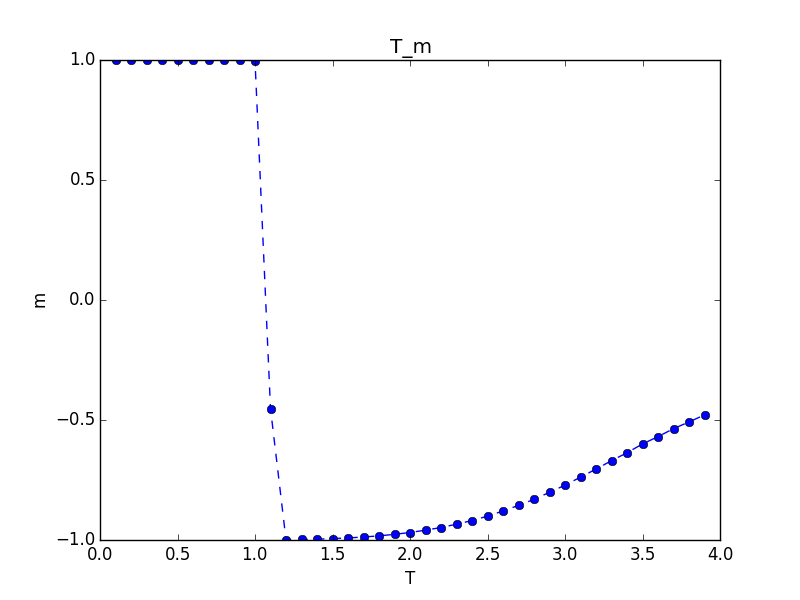
\includegraphics[width = 5cm]{T_m_128_J1_H-0.5.png}}
        \subfigure[J=1,H=0]{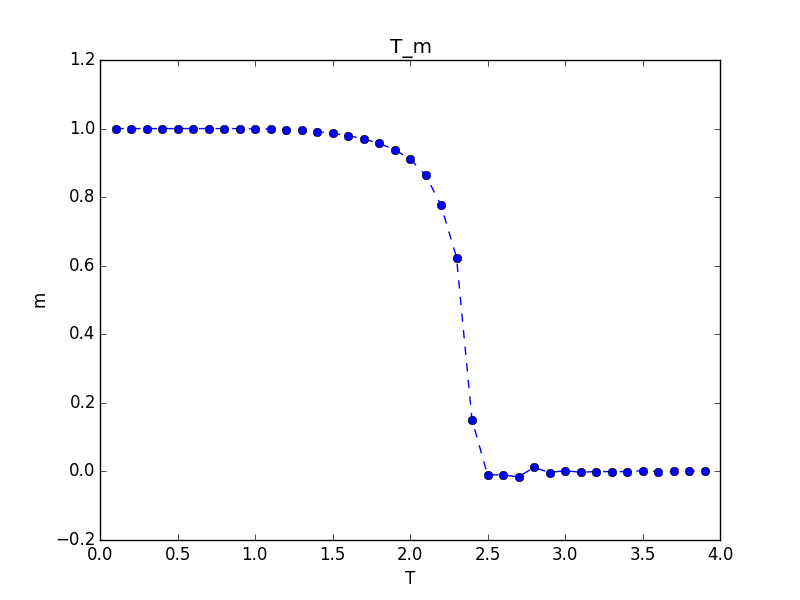
\includegraphics[width = 5cm]{T_m_128_J1_H0.png}}
        \subfigure[J=1,H=0.5]{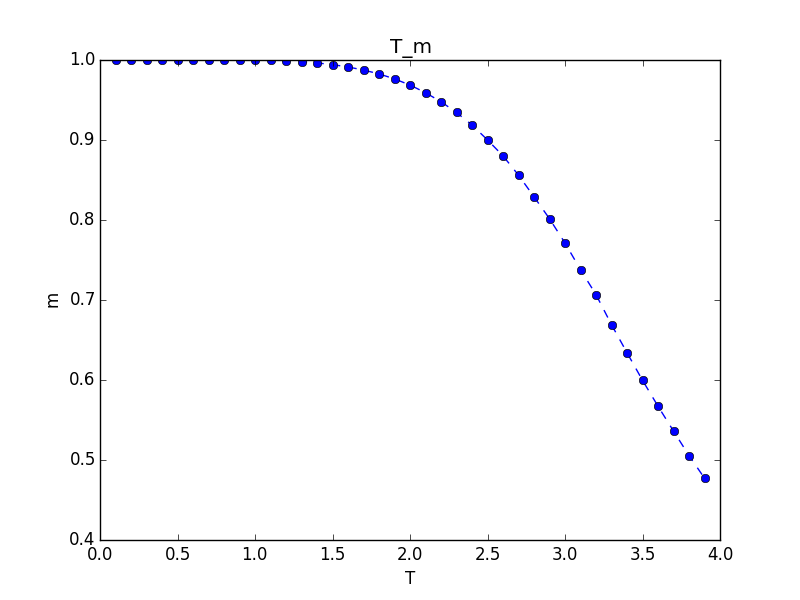
\includegraphics[width = 5cm]{T_m_128_J1_H0.5.png}}
    \end{center}
\end{figure}

\paragraph{改变磁场,E随T的变化趋势改变}

\begin{figure}[hbt]
    \caption{E\_T趋势随磁场变化}
    \setcounter{subfigure}{0}
    \begin{center}
        \subfigure[J=1,H=-0.5]{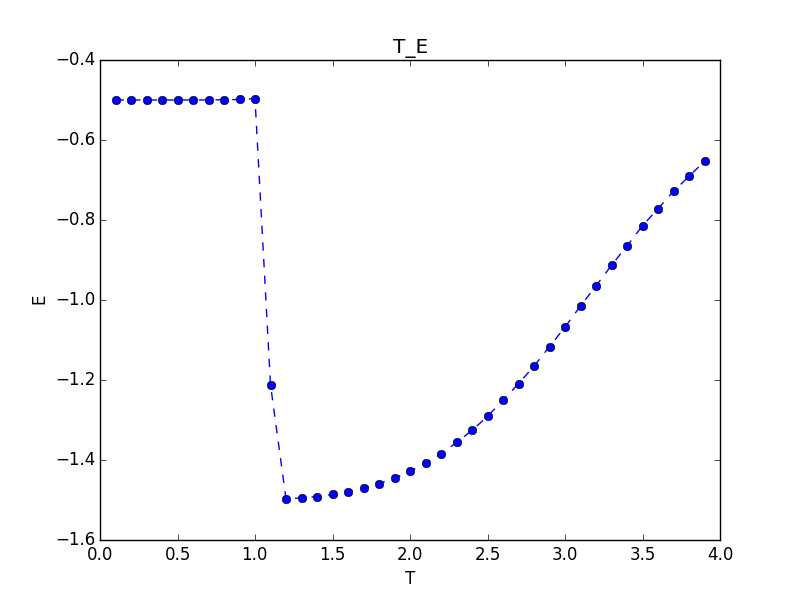
\includegraphics[width = 5cm]{T_E_128_J1_H-0.5.png}}
        \subfigure[J=1,H=0]{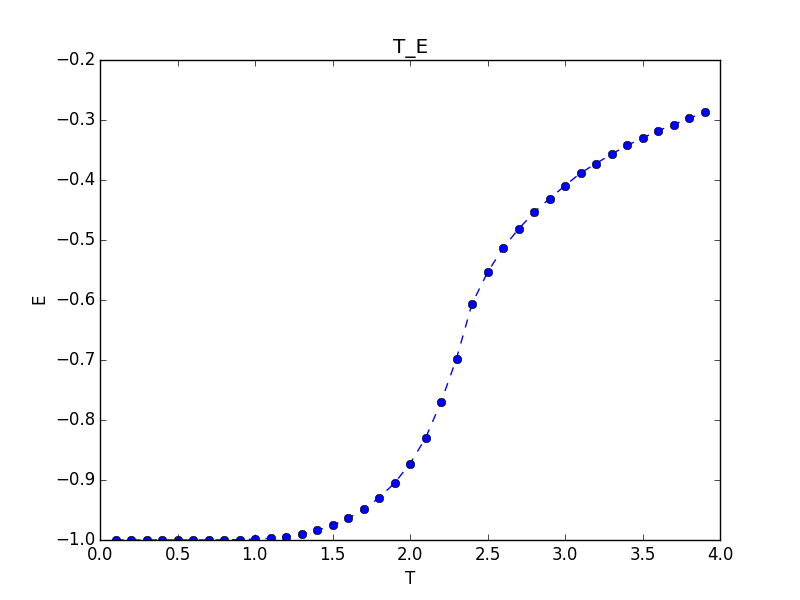
\includegraphics[width = 5cm]{T_E_128_J1_H0.png}}
        \subfigure[J=1,H=0.5]{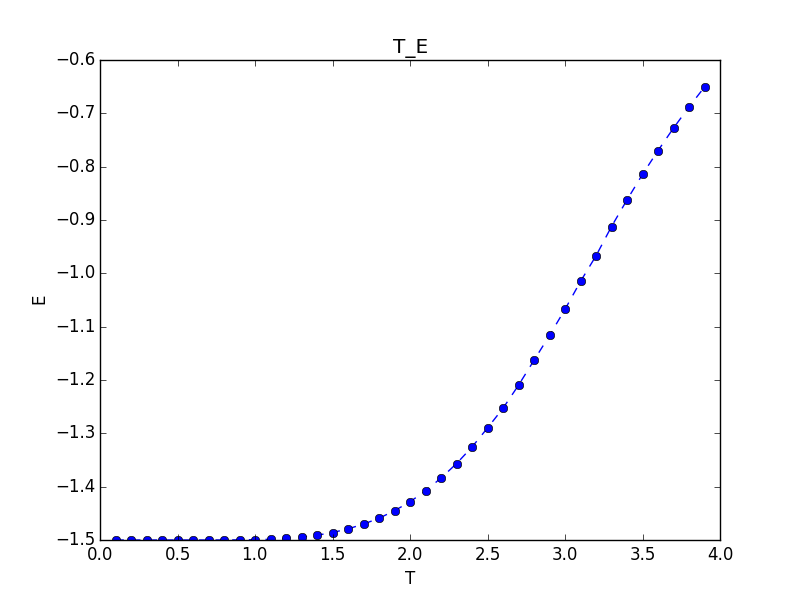
\includegraphics[width = 5cm]{T_E_128_J1_H0.5.png}}
    \end{center}
\end{figure}

\clearpage
\paragraph{改变温度,m随H的变化趋势改变}
\begin{figure}[hbt]
    \caption{m\_H趋势随温度变化}
    \setcounter{subfigure}{0}
    \begin{center}
        \subfigure[T=1,J=1]{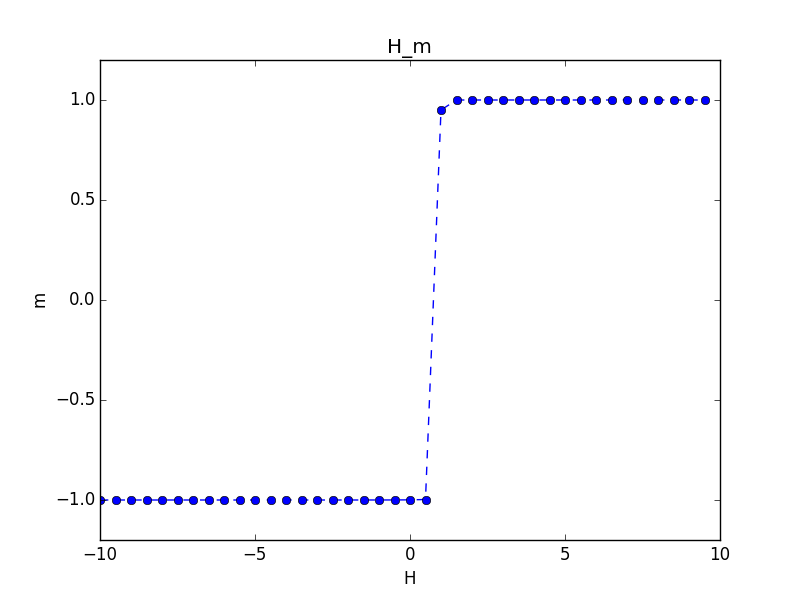
\includegraphics[width = 5cm]{H_m_128_T1_J1.png}}
        \subfigure[T=2.25,J=1]{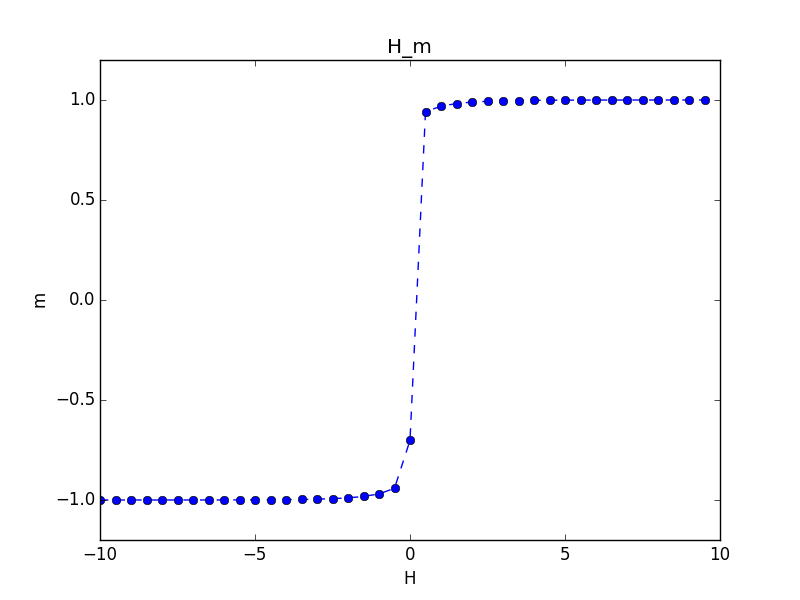
\includegraphics[width = 5cm]{H_m_128_T2.25_J1.png}}
        \subfigure[T=4,J=1]{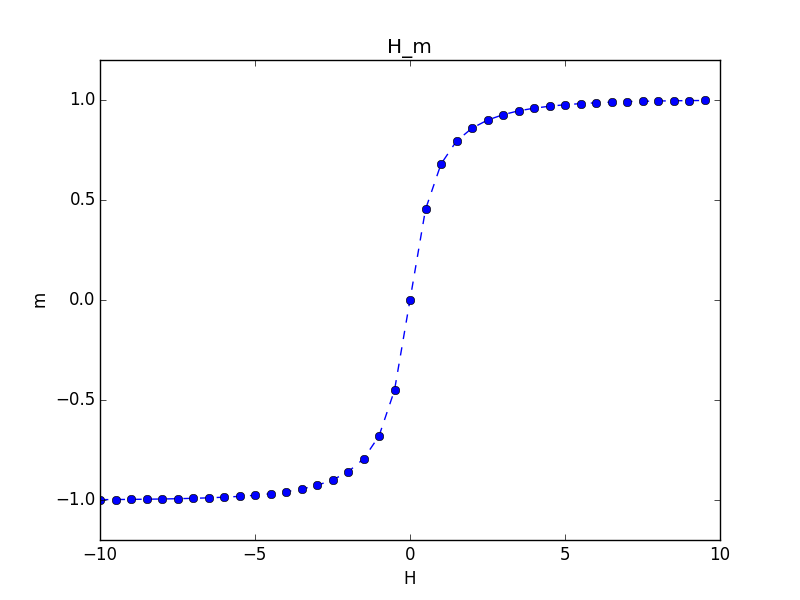
\includegraphics[width = 5cm]{H_m_128_T4_J1.png}}
    \end{center}
\end{figure}

\paragraph{改变温度,E随H的变化趋势改变}
\begin{figure}[hbt]
    \caption{E\_H趋势随温度变化}
    \setcounter{subfigure}{0}
    \begin{center}
        \subfigure[T=1,J=1]{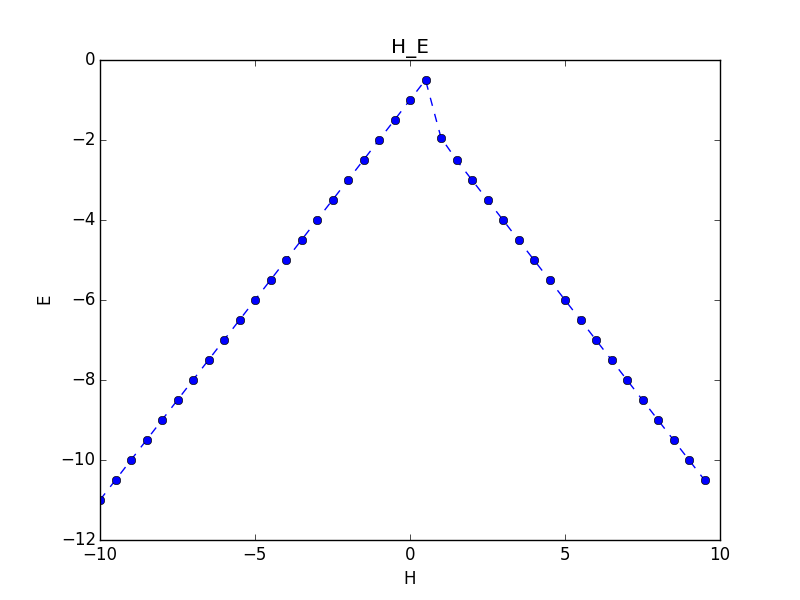
\includegraphics[width = 5cm]{H_E_128_T1_J1.png}}
        \subfigure[T=2.25,J=1]{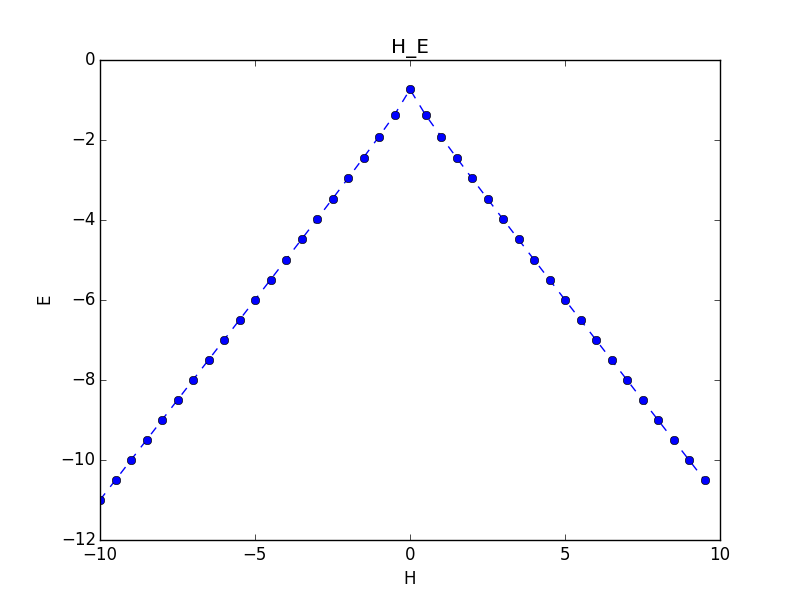
\includegraphics[width = 5cm]{H_E_128_T2.25_J1.png}}
        \subfigure[T=4,J=1]{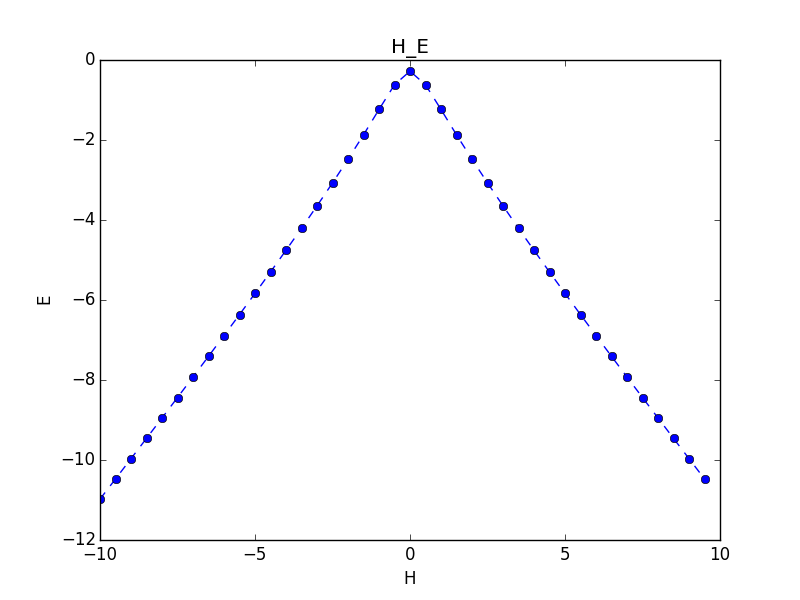
\includegraphics[width = 5cm]{H_E_128_T4_J1.png}}
    \end{center}
\end{figure}

\clearpage
\subsubsection{磁滞回线}
当对磁场H为一级相变时,演增大和减小磁场的方向改变磁场:
\begin{figure}[hbt]
    \caption{磁滞回线}
    \begin{center}
        \subfigure[T=1,J=1]{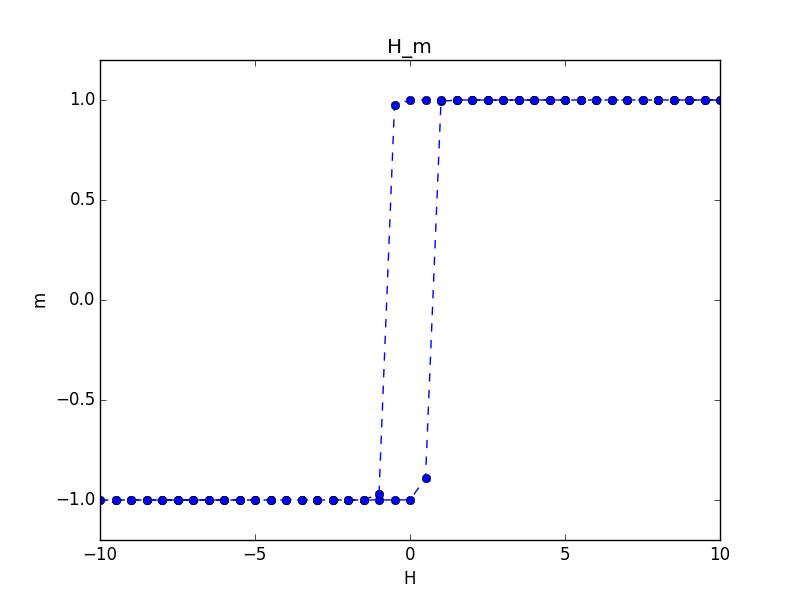
\includegraphics[width = 5cm]{Loop_H_m_128_T1_J1.png}}
        \subfigure[T=2.25,J=1]{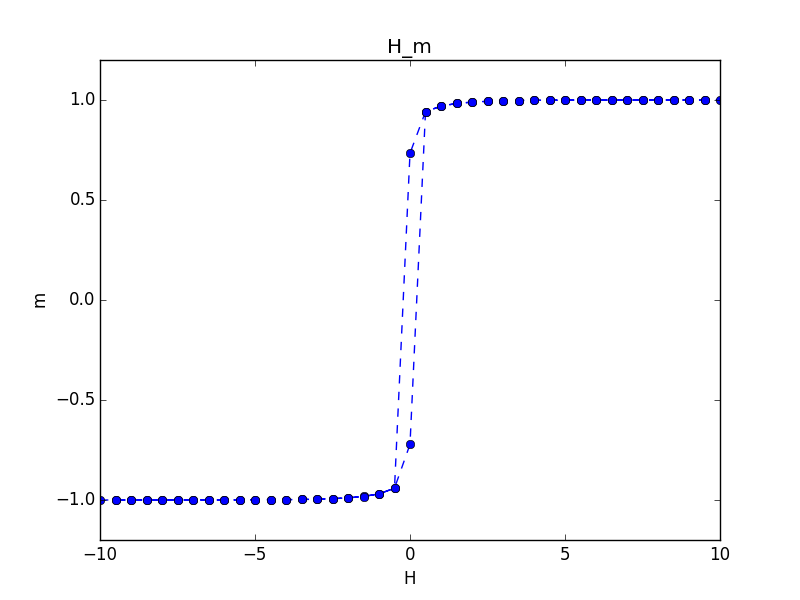
\includegraphics[width = 5cm]{Loop_H_m_128_T2.25_J1.png}}
        \subfigure[T=4,J=1]{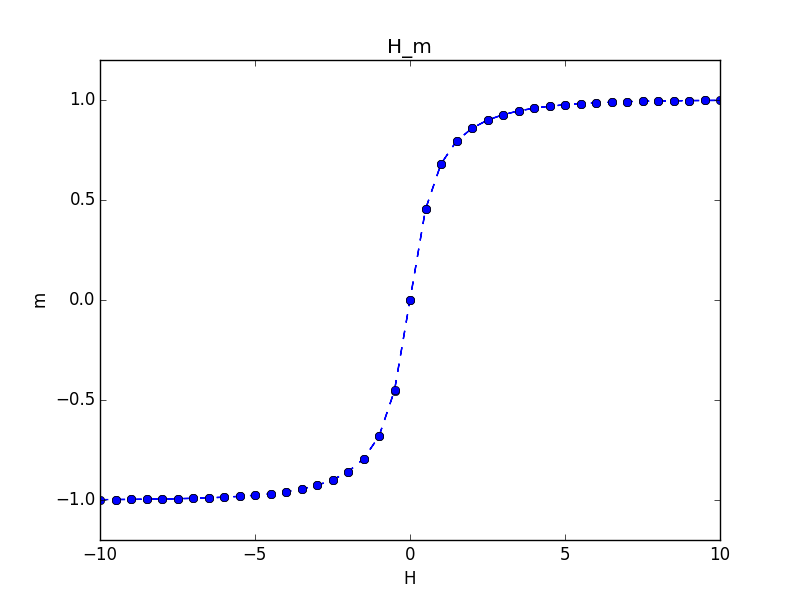
\includegraphics[width = 5cm]{Loop_H_m_128_T4_J1.png}}
    \end{center}
\end{figure}
不难发现,磁滞回线随着温度的增高逐渐消失,这是因为在模拟中自旋反转的机率正比于$\exp(-\Delta E/k_{B}T)$,T越小,该机率越小,系统处于亚稳态的惯性越强,故更倾向于留在原来态.这样从正反方向演化,也就出现了相变点的不同,进而产生了磁滞回线.

\section{总结}
概要的介绍了Ising模型,并用Monte Carlo方法对二维Ising模型进行了模拟,讨论了稳态组态,一级相变,二级相变等若干问题.
Ising模型是统计物理中同时具备了:表述简单,内涵丰富,应该广泛三种有点.
其扩展模型有:
\begin{enumerate}
    \item XY模型: 自旋可以在平面中任意取向.
    \item Heisenberg模型: 自旋在三维空间中任意去向.
    \item Potts模型:自旋不再是$\pm1$而是可以取q个离散状态.
    \item 时钟模型: 二维中间中q个离散取向(XY模型+Potts模型)
    \item Ising自旋玻璃: Ising模型中$J_{ij}$取满足Gauss分布的随机变量.
\end{enumerate}
相关的应用也有很多,比如磁化模拟,投票模型,神经网络模型等.

\clearpage
\renewcommand\refname{参考文献}
\begin{thebibliography}{99}

    \bibitem{Ising_wiki}
        https://en.wikipedia.org/wiki/Ising\_model

    \bibitem{热统汪志诚}
        汪志诚. 热力学·统计物理[M]// 高等教育出版社, 2008.第九章 9.5

    \bibitem{Metropolis_wiki}
        https://en.wikipedia.org/wiki/Metropolis–Hastings\_algorithm\#cite\_note-Metropolis-1

    \bibitem{Metropolis:1953vj}
        Metropolis, N., Rosenbluth, A. W., Rosenbluth, M. N., Teller, A. H. \& Teller, E. Equation of State Calculations by Fast Computing Machines. The Journal of Chemical Physics 21, 1087–1092 (1953).

    \bibitem{Master_equ}
        https://en.wikipedia.org/wiki/Master\_equation

    \bibitem{Swendsen:1987eq}
        Swendsen, R. H. \& Wang, J.-S. Nonuniversal critical dynamics in Monte Carlo simulations. Phys. Rev. Lett. 58, 86–88 (1987).

    \bibitem{Hoshen:1976vg}
        Percolation and cluster distribution. I. Cluster multiple labeling technique and critical concentration algorithm. (1976).

    \bibitem{Wolff:1988uh}
        Ulli Wolff. Collective Monte Carlo Updating for Spin Systems. 62, 361–364. 15 p (1989).

    \bibitem{Krauth:2003ts}
        Krauth, W. Cluster Monte Carlo algorithms. arXiv cond-mat.stat-mech, (2003).

\end{thebibliography}

\end{document}
